% Template for PLoS
% Version 3.4 January 2017
%
% % % % % % % % % % % % % % % % % % % % % %
%
% -- IMPORTANT NOTE
%
% This template contains comments intended 
% to minimize problems and delays during our production 
% process. Please follow the template instructions
% whenever possible.
%
% % % % % % % % % % % % % % % % % % % % % % % 
%
% Once your paper is accepted for publication, 
% PLEASE REMOVE ALL TRACKED CHANGES in this file 
% and leave only the final text of your manuscript. 
% PLOS recommends the use of latexdiff to track changes during review, as this will help to maintain a clean tex file.
% Visit https://www.ctan.org/pkg/latexdiff?lang=en for info or contact us at latex@plos.org.
%
%
% There are no restrictions on package use within the LaTeX files except that 
% no packages listed in the template may be deleted.
%
% Please do not include colors or graphics in the text.
%
% The manuscript LaTeX source should be contained within a single file (do not use \input, \externaldocument, or similar commands).
%
% % % % % % % % % % % % % % % % % % % % % % %
%
% -- FIGURES AND TABLES
%
% Please include tables/figure captions directly after the paragraph where they are first cited in the text.
%
% DO NOT INCLUDE GRAPHICS IN YOUR MANUSCRIPT
% - Figures should be uploaded separately from your manuscript file. 
% - Figures generated using LaTeX should be extracted and removed from the PDF before submission. 
% - Figures containing multiple panels/subfigures must be combined into one image file before submission.
% For figure citations, please use "Fig" instead of "Figure".
% See http://journals.plos.org/plosone/s/figures for PLOS figure guidelines.
%
% Tables should be cell-based and may not contain:
% - spacing/line breaks within cells to alter layout or alignment
% - do not nest tabular environments (no tabular environments within tabular environments)
% - no graphics or colored text (cell background color/shading OK)
% See http://journals.plos.org/plosone/s/tables for table guidelines.
%
% For tables that exceed the width of the text column, use the adjustwidth environment as illustrated in the example table in text below.
%
% % % % % % % % % % % % % % % % % % % % % % % %
%
% -- EQUATIONS, MATH SYMBOLS, SUBSCRIPTS, AND SUPERSCRIPTS
%
% IMPORTANT
% Below are a few tips to help format your equations and other special characters according to our specifications. For more tips to help reduce the possibility of formatting errors during conversion, please see our LaTeX guidelines at http://journals.plos.org/plosone/s/latex
%
% For inline equations, please be sure to include all portions of an equation in the math environment.  For example, x$^2$ is incorrect; this should be formatted as $x^2$ (or $\mathrm{x}^2$ if the romanized font is desired).
%
% Do not include text that is not math in the math environment. For example, CO2 should be written as CO\textsubscript{2} instead of CO$_2$.
%
% Please add line breaks to long display equations when possible in order to fit size of the column. 
%
% For inline equations, please do not include punctuation (commas, etc) within the math environment unless this is part of the equation.
%
% When adding superscript or subscripts outside of brackets/braces, please group using {}.  For example, change "[U(D,E,\gamma)]^2" to "{[U(D,E,\gamma)]}^2". 
%
% Do not use \cal for caligraphic font.  Instead, use \mathcal{}
%
% % % % % % % % % % % % % % % % % % % % % % % % 
%
% Please contact latex@plos.org with any questions.
%
% % % % % % % % % % % % % % % % % % % % % % % %

\documentclass[10pt,letterpaper]{article}
\usepackage[top=0.85in,left=2.75in,footskip=0.75in]{geometry}
\usepackage{graphicx}
\graphicspath{ {figures/} }

% amsmath and amssymb packages, useful for mathematical formulas and symbols
\usepackage{amsmath,amssymb}

% Use adjustwidth environment to exceed column width (see example table in text)
\usepackage{changepage}

% Use Unicode characters when possible
\usepackage[utf8x]{inputenc}

% textcomp package and marvosym package for additional characters
\usepackage{textcomp,marvosym}

% cite package, to clean up citations in the main text. Do not remove.
\usepackage{cite}

% Use nameref to cite supporting information files (see Supporting Information section for more info)
\usepackage{nameref,hyperref}

% line numbers
\usepackage[right]{lineno}

% ligatures disabled
\usepackage{microtype}
\DisableLigatures[f]{encoding = *, family = * }

% color can be used to apply background shading to table cells only
\usepackage[table]{xcolor}
\definecolor{Gray}{gray}{0.45}
\definecolor{LightGray}{gray}{0.9}
\definecolor{VeryLightGray}{gray}{0.93}
\definecolor{LightCyan}{rgb}{0.88,1,1}
\definecolor{Goldenrod}{rgb}{0.95,0.95,0.9}

% array package and thick rules for tables
\usepackage{array}

%further packages (not from PLoS template)
\usepackage{csvsimple}

% create "+" rule type for thick vertical lines
\newcolumntype{+}{!{\vrule width 2pt}}

% create \thickcline for thick horizontal lines of variable length
\newlength\savedwidth
\newcommand\thickcline[1]{%
  \noalign{\global\savedwidth\arrayrulewidth\global\arrayrulewidth 2pt}%
  \cline{#1}%
  \noalign{\vskip\arrayrulewidth}%
  \noalign{\global\arrayrulewidth\savedwidth}%
}

% \thickhline command for thick horizontal lines that span the table
\newcommand\thickhline{\noalign{\global\savedwidth\arrayrulewidth\global\arrayrulewidth 2pt}%
\hline
\noalign{\global\arrayrulewidth\savedwidth}}


% Remove comment for double spacing
%\usepackage{setspace} 
%\doublespacing

% Text layout
\raggedright
\setlength{\parindent}{0.5cm}
\textwidth 5.25in 
\textheight 8.75in

% Bold the 'Figure #' in the caption and separate it from the title/caption with a period
% Captions will be left justified
\usepackage[aboveskip=1pt,labelfont=bf,labelsep=period,justification=raggedright,singlelinecheck=off]{caption}
\renewcommand{\figurename}{Fig}

% Use the PLoS provided BiBTeX style
\bibliographystyle{plos2015}

% Remove brackets from numbering in List of References
\makeatletter
\renewcommand{\@biblabel}[1]{\quad#1.}
\makeatother

% Leave date blank
\date{}

% Header and Footer with logo
\usepackage{lastpage,fancyhdr,graphicx}
\usepackage{epstopdf}
\pagestyle{myheadings}
\pagestyle{fancy}
\fancyhf{}
\setlength{\headheight}{27.023pt}
\lhead{
\includegraphics[width=2.0in]{PLOS-submission.eps}}
\rfoot{\thepage/\pageref{LastPage}}
\renewcommand{\footrule}{\hrule height 2pt \vspace{2mm}}
\fancyheadoffset[L]{2.25in}
\fancyfootoffset[L]{2.25in}
\lfoot{\sf PLOS}

%% Include all macros below

\newcommand{\lorem}{{\bf LOREM}}
\newcommand{\ipsum}{{\bf IPSUM}}

%% END MACROS SECTION


\begin{document}
\vspace*{0.2in}

% Title must be 250 characters or less.
\begin{flushleft}
{\Large
\textbf\newline{Using phenotype prediction to explore the functional capabilities of metagenomically assembled microbial genomes} % Please use "sentence case" for title and headings (capitalize only the first word in a title (or heading), the first word in a subtitle (or subheading), and any proper nouns).
}
\newline
% Insert author names, affiliations and corresponding author email (do not include titles, positions, or degrees).
\\
Fred Farrell\textsuperscript{1*},
Orkun S. Soyer\textsuperscript{1},
Christopher Quince\textsuperscript{2},
\\
\bigskip
\textbf{1} School of Life Sciences, University of Warwick, Coventry, United Kingdom
\\\textbf{2} Warwick Medical School, University of Warwick, Coventry, United Kingdom
\\
%\textbf{3} Affiliation Dept/Program/Center, Institution Name, City, State, Country
%\\
\bigskip

% Insert additional author notes using the symbols described below. Insert symbol callouts after author names as necessary.
% 
% Remove or comment out the author notes below if they aren't used.
%
% Primary Equal Contribution Note
%\Yinyang These authors contributed equally to this work.

% Additional Equal Contribution Note
% Also use this double-dagger symbol for special authorship notes, such as senior authorship.
%\ddag These authors also contributed equally to this work.

% Current address notes
%\textcurrency Current Address: Dept/Program/Center, Institution Name, City, State, Country % change symbol to "\textcurrency a" if more than one current address note
% \textcurrency b Insert second current address 
% \textcurrency c Insert third current address

% Deceased author note
%\dag Deceased

% Group/Consortium Author Note
%\textpilcrow Membership list can be found in the Acknowledgments section.

% Use the asterisk to denote corresponding authorship and provide email address in note below.
* f.farrell@warwick.ac.uk

\end{flushleft}
% Please keep the abstract below 300 words
\section*{Abstract}
Using machine learning, we predict functional and metabolic traits of bacteria and archaea from their genomes. To train these models, we use a database of 84 phenotypic traits associated with 9407 prokaryotic genomes downloaded from the NCBI genome database. We compared multiple models and choices of feature vectors. We found that a lasso logistic regression using frequency of KEGG orthologs performed best. This model was able to classify 65 of these functions with greater than 90\% cross-validated AUROC score. We then used this models to predict the phenotypes of novel microbial genomes assembled from metagenomic studies from a variety of environments.


% Please keep the Author Summary between 150 and 200 words
% Use first person. PLOS ONE authors please skip this step. 
% Author Summary not valid for PLOS ONE submissions.   
%\section*{Author summary}
%Lorem ipsum dolor sit amet, consectetur adipiscing elit. Curabitur eget porta erat. Morbi consectetur est vel gravida pretium. Suspendisse ut dui eu ante cursus gravida non sed sem. Nullam sapien tellus, commodo id velit id, eleifend volutpat quam. Phasellus mauris velit, dapibus finibus elementum vel, pulvinar non tellus. Nunc pellentesque pretium diam, quis maximus dolor faucibus id. Nunc convallis sodales ante, ut ullamcorper est egestas vitae. Nam sit amet enim ultrices, ultrices elit pulvinar, volutpat risus.

\linenumbers

% Use "Eq" instead of "Equation" for equation citations.
\section*{Introduction}
The increasing ease of genetic sequencing has led to an explosion in the amount of such data generated. In the context of microbial ecology, large-scale metagenomic studies such as the Human Microbiome Project~\cite{Huttenhower2012}, the Earth Microbiome Project~\cite{Gilbert2014} and the Tara Oceans Project~\cite{Zhang2015} have systematically sequenced the microbial communities in a huge variety of environments at great depth. Amplicon sequencing, such as of the 16S rRNA gene, allows detailed study of the taxonomic makeup of these communities, while shotgun metagenomic sequencing allows characterisation of all genes present in an environment. Increasing depth of coverage and improvements in genome binning algorithms for clustering contigs into genomes, in particular the use of differential coverage across different samples~\cite{Alneberg2014, Eren2015}, are allowing more and more full and partial genomes to be assembled from shotgun metagenomic studies. Many of these organisms are novel and uncultured, having never been studied in a lab. A recent metagenomic study on aquifer systems~\cite{Anantharaman2016}, for example, reconstructed 2540 separate high-quality, near-complete genomes, and claimed to have discovered an astonishing 47 new phylum-level lineages among them.

Interpretation of these results is time-consuming and difficult, and cannot keep up with the rate of data being generated. In particular, we would like to know the phenotypic traits and, hence, ecological roles, of these novel organisms, many of which will have no cultured relatives. As such, automated ways to associate genomic data with phenotypic features are required. There are a variety of tools and databases for annotating genes in genomes e.g. the Kyoto Encyclopedia of Genes and Genomes (KEGG)~\cite{Kanehisa2017}, the Pfam database of protein families~\cite{Finn2016} and the NCBI COG database of orthologous genes~\cite{Tatusov1997}. These functional annotations are often associated with higher level metabolic pathways in the databases but converting these to an actual prediction of 
phenotype still relies on manually studying particular genes of interest in a time consuming process whose accuracy is not easily quantifiable.

%There are automated tools for interfacing with these databases, for example %PICRUSt~\cite{Langille2013}, which performs ancestral state reconstruction to link 16S %sequences with full genomes using the KEGG orthology. 

In the interest of developing a way to automatically gain an overview of phenotypic and functional characteristics associated with the results of metagenomic studies, we here present a method of using existing knowledge of phenotypes associated with microbial taxa to make predictions about new organisms based on their genomes.

To do this, we utilised a recently published database, the FAPROTAX database~\cite{Louca2016,Louca2017}, of phenotypes known to be associated with certain microbial taxa, based on an extensive survey of the scientific literature. The aim of creating this database was to allow microbes found from 16S rRNA amplicon sequencing to be assigned into functional and metabolic groups, so that functional variation across environemnts could be studied and compared to taxonomic variation. The authors found that abundance of functional groups was strongly influenced by environmental conditions in a variety of ocean environments~\cite{Louca2016a}. The bulk of the classifications in the FAPROTAX database come from \emph{Bergey's Manual of Systematic Bacteriology}~\cite{Whitman}, and it currently contains 84 phenotypic traits associated with 4600 microbial taxonomic groups. We wanted to allow the information contained in the database to be used to analyse novel genomes produced in shotgun sequencing studies, giving us the ability to make predictions about their functional roles. To do this, we combined this existing database with genomes downloaded from the NCBI and used machine learning to train statistical models able to infer an organism's traits from a vector of 
genes annotated to functional groups. Machine learning techniques, such as logistic regression and support vector machines (SVMs) have previously been used in bioinformatics to infer phenotypic information from gene sequences, for example using SVMs on amino acid k-mer frequencies to predict protein function~\cite{Leslie2002,Cai2003,Someya2010}. A recent paper~\cite{Asgari2015} achieved good results in this task with recurrent neural networks, which can classify proteins directly from their sequences without the need for feature extraction. 

Here, we use the presence of known gene orthologs, for example from the KEGG database, to train models of the phenotype of whole organisms. This work was inspired by a recent software famework, Traitar~\cite{Weimann2016}, which uses SVMs to predict microbial traits based on genomic information in the form of copy numbers of Pfam families. Our work differs from Traitar in the use of the highly detailed FAPROTAX database. Traitar utilised the Global Infectious Disease and Epidemiology Online Network (GIDEON)~\cite{Berger2005} for its phenotypic annotations, and was therefore biased toward pathogenic traits; we instead focus on traits associated with metabolism and environmental niche. Additionally, we have a significantly larger training set---genomes from all 9407 unique species having a genome classified as `full' in the NCBI database---whereas Traitar used 234. The size of the training set is usually expected to have significant impact on the performance of a machine learning model.

We show that models so trained have a good accuracy at determining the phenotype of an unknown species over many functions, with 65 functions out of 84 achieving an AUROC score above 90\%. In particular, in many cases the classification accuracy is superior to using manually-curated `KEGG modules', which are small groups of genes in the KEGG database known to be associated with a particular function. We also compare the performance of a variety of machine learning models at this task, and of using two different genome annotation frameworks, the KEGG ortholog scheme and the Pfam protein family database. 

We then go on to use these models to predict the phenotypes of so-called MAGs (metagenome assembled genomes), genomes assembled from metagenomic studies and otherwise unstudied, from three diverse environments: anaerobic digesters, ground water aquifers and the ocean.  


\section*{Materials and methods}
\subsection*{Databases and preparation of training data}
To train our models, we utilized the combination of the recently-published FAPROTAX database of microbial phenotypes and the NCBI genome database. We downloaded all prokaryotic genomes classified as `full' from the NCBI Genome database. We used the taxonomic information available from NCBI to assign them phenotypes using the script `collapse\_table.py' which comes as part of the FAPROTAX database~\cite{Louca2016}. We then called genes in these genomes using Prodigal~\cite{Hyatt2010}. We annotated the resulting inferred coding DNA sequences (CDS) both by aligning against against the KEGG database using Diamond BLASTP~\cite{Buchfink2014} and by searching with hmmer3~\cite{Eddy2011} against Pfam~\cite{Finn2016}. The result is a matrix of organisms and and their copy numbers of either KEGG orthologs or Pfam domains. We have found that using gene copy number rather than simple presence/absence significantly increases classifier performance. The scripts we used to download and process the genomes are available at ...

\subsection*{Statistical modelling}
To model the link between genotype, in the form of KEGG ortholog copy numbers or Pfam protein families, and phenotype as represented in the FAPROTAX database, we used a variety of machine learning techniques. These are all different ways of learning the relationship between the features (gene copy numbers) and targets (biological functions) from the training data of 9407 NCBI genomes from unique species. To train the algorithms, we first split this data into a training set (75\% of the genomes) and a test set (25\%), by random sampling. The algorithms were then trained on the training data, and their performance tested on the unseen test data genomes, to check that the relationships learned are generalisable (i.e. that the algorithms have not `overfit' the training data). Below, we describe the algorithms used.

\subsubsection*{Logisic regression}
We found logistic regression, a commonly used linear model used for classification problems,~\cite{Hastie2009a,Freedman2009} to be very useful in our case. The genome dataset was split into a training set and a testing set, for testing the performance of the algorithm on unseen data. Additionally, we scaled all input features to have mean zero and variance 1 before performing the regression. Since the number of KEGG orthologs (features) was somewhat larger than the number of training examples, overfitting, whereby the model classifies on features of the training set which are very specific to it, was a serious problem. To alleviate this, we used logistic regression with an $\ell$1 penalty term, also known as LASSO logistic regression~\cite{Lee2006}, whereby large parameters are penalized in such a way that only a few of the features have a nonzero weight. In detail, the method involves adding a penalty term equal to the $\ell$1-norm of all of the coefficients of the regressor, thereby penalising nonzero terms, so that the optimization problem becomes:
\begin{equation}
\min_{w}\left[||w||_1 + C\sum_{i=1}^{n}\log\left(\exp(-y_i(X_i^T w )) + 1\right)\right]
\end{equation}
where $w$ is the vector of regression weights, $X_i$ are the feature vectors of each example, $y_i$ the classification targets, and $C$ is a parameter defining the (inverse) strength of the regularization. This method of regularization is often useful in cases where the number of features is large (similar to or larger than the number of training examples), as most of the features are not used in the classification task. For example, a recent study used $\ell$1-regularized regression to predict complex human traits such as height and heel-bone density from a large array of SNPs (around 100000), significantly improving on previous estimates of heritability based on individual SNPs~\cite{Lello2017}. 

%In our case, we found that this method significantly outperformed other commonly-used and %somewhat more complex classification algorithms, such as random forests and support %vector machines.

\subsubsection*{Random forests}
We also used the random forest algorithm, a popular machine learning method which can be applied to both regression and classification problems, is simple to use, fast and performs fairly well on a wide variety of problems~\cite{Hastie2009}. The random forest is an `ensemble' method, using a collection of slightly randomized classifiers, the results of which are averaged to produce a prediction. This helps to avoid overfitting. A random forest in particular is an ensemble of so-called decision trees. A decision tree is a model which learns to split up training examples into sets according to their feature values, with the aim of separating the target classes. They have the advantage of being invariant under scaling of features and adding irrelevant features, this last feature being useful in our case where the number of features is very large and many are irrelevant to the classification task; they can also learn more complex relationships between variables than a linear model such as logistic regression. However, they tend to overfit the training data. A random forest trains a large number of such trees on random subsets of the features and combines these predictions by averaging, much improving performance. 

\subsubsection*{Support vector machines}
Finally, we used support vector machines (SVMs)~\cite{Hastie2009b}. An SVM essentially tries to find surfaces in the high-dimensional feature space which separate the different classes as well as possible, and with as wide a margin as possible between the surface and the examples. These surfaces can be either linear or non-linear (if a non-linear kernel is used); they are therefore capable of learning complex non-linear relationships between features and targets. They can also include regularization terms as in logistic regression, to reduce overfitting. 


\subsection*{Metrics and classifier performance}
Since many of the classes which we are attempting to predict are highly unbalanced (e.g. of the 9407 unique species with full genomes in the NCBI database only 83 are hydrogentotrophic methanogens), simple classification accuracy is not a very useful measure of classifier performance. Predicting all labels as negative in the above example would give an accuracy of 99.1\% despite not being a useful classifier. We therefore need a metric which can take into account class imbalance. We use the area under the ROC (Receiver Operating Characteristic) curve, which is a graph of true postive rate against false positive rate as one varies the cutoff in probability for making a positive prediction~\cite{Fawcett2006,Flach2011}. An AUROC score much greater than 0.5 (the score for random predictions) indicates a good classifier. In particular, a score of 1 indicates that all positive cases have been assigned a higher probability than all negative cases.

\subsection*{Prediction of MAG phenotypes}
Once classifiers have been trained on the NCBI data, it is possible to use them to make predictions about unseen genomes, such as MAGs generated from shotgun sequencing studies. The MAGs must first be processed to give a matrix of the KEGG ortholog copy numbers associated with them, using the same pipeline applied above the NCBI genomes. These matrices are then used as input into the classifiers to produce a matrix of MAGs and their predicted functions, which can be either presence/absence predictions or probabilities. 


% Results and Discussion can be combined.
\section*{Results}
\subsection*{Classification accuracy}
Figure~\ref{fig1} shows the performance of the algorithm in the classification task on the test set in terms of AUROC (area under the Receiver Operating Characteristic, see Materials and Methods) score. The accuracies were calculated using k-fold cross-validation with $k=5$, i.e. the data was split into training and testing sets 5 times, in such a way that each training example was in the test set once, and the prediction for each data point when it was in the test set was used.  The results are shown for two classification algorithms, $\ell$1-regularized logistic regression and the random forest. The regularized logistic regression performs significantly better for many, though not all, functions. The average score over all functions for LR is 90.1\% (versus 84.5\% for the random forest), and 65 functions have a score greater than 90\%, with 45 higher than 95\%.

% Place figure captions after the first paragraph in which they are cited.
\begin{figure}[!h]
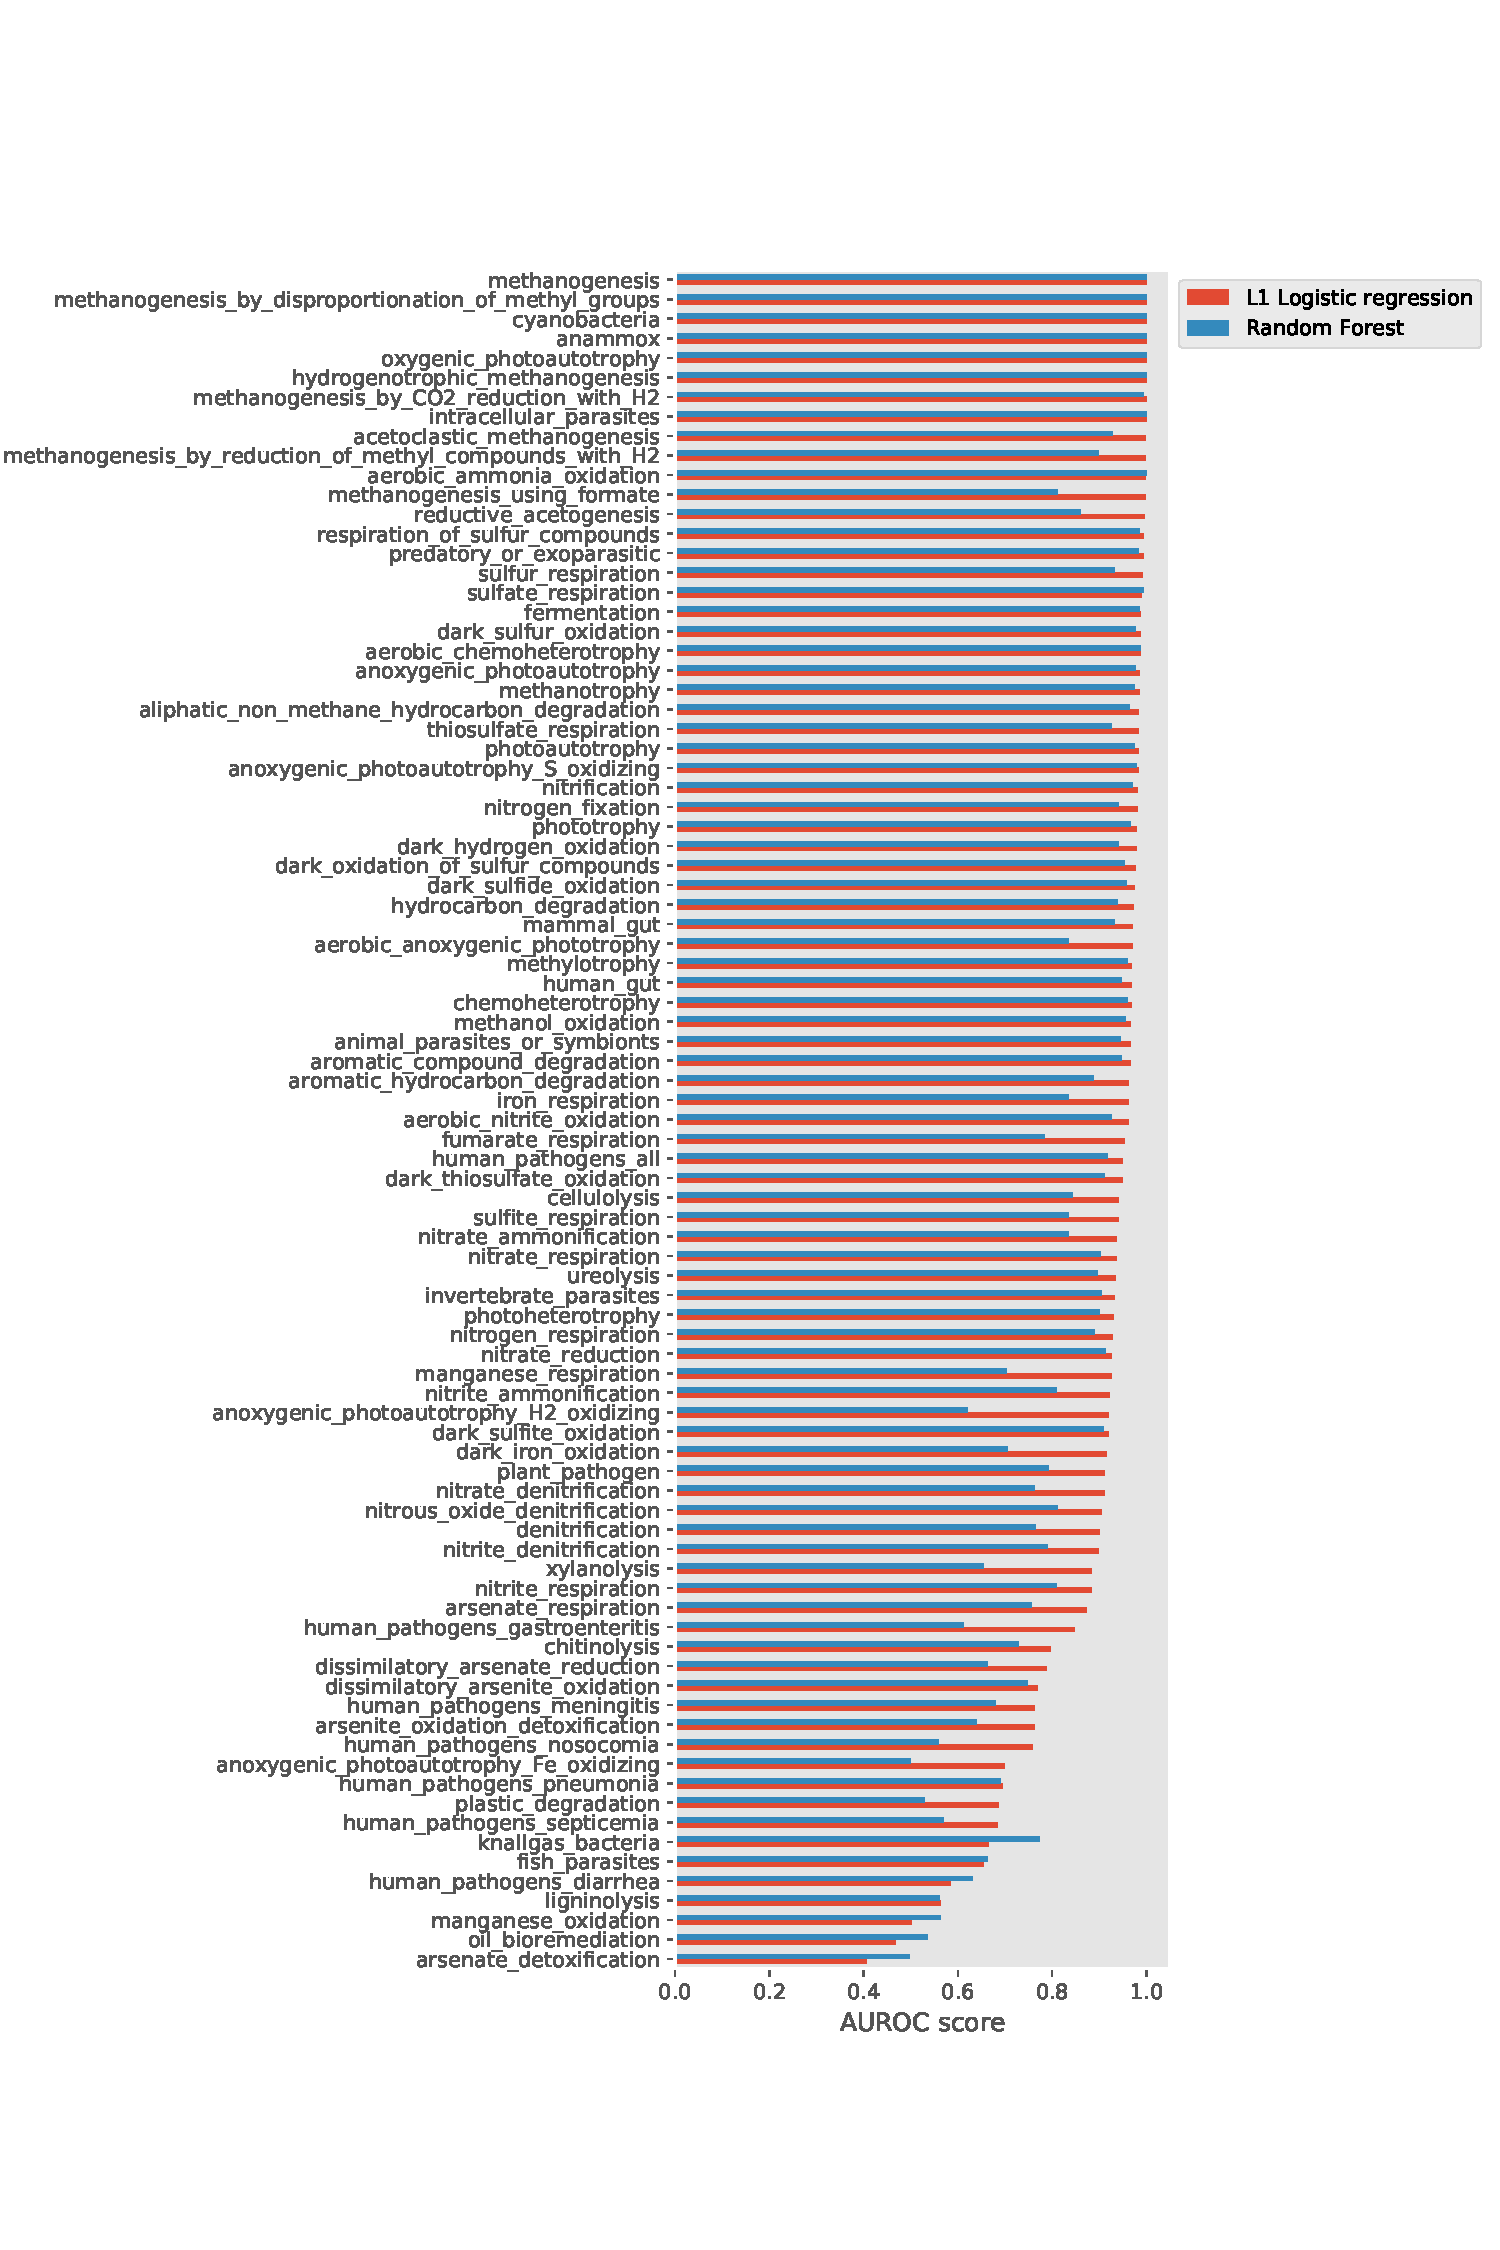
\includegraphics[width=0.9\textwidth]{fig1}
\caption{{\bf Overall performance of classification algorithms.}
The AUROC score on each classification task (each function) is shown for two classification algorithms: $\ell$1-regularized logistic regression and the random forest. Functions are ordered by the LR score.}
\label{fig1}
\end{figure}


\subsection*{Gene orthologs used by classifiers}
Table~\ref{tab1} shows the KEGG orthologs with non-zero coefficients used by the LR classifiers and their weights for some example functions. Due to the $\ell1$-regularization, the number of non-zero coefficients is rather low. Three representative functions, all having classifiers with AUROC scores greater than 95\%, are shown. Many of the KEGG orthologs picked out by the classifiers are genes known to be involved in these functions, as we might hope. In particular, consider the prediction of methanogens, a relatively easy task since it is known that methanogens must possess the \emph{mcrA} gene, this being a necessary and sufficient condition for methanogenesis [REF]. Indeed, subunits of this gene have the highest weight, and a total of only 9 genes are used by the classifier. 

Looking at some more complex traits, for example sulfate respiration (i.e. disimmilatory sulfate reduction to H$_{2}$S), the model assigns a lot of weight to subunits of a quinone-modifying oxidoreductase, which is indeed associated with sulfur metabolism [REF]. Interestingly, however, none of the genes picked out by the classifier are directly part of the metabolic pathway for this process as described in the KEGG module for dissimilatory sulfate reduction, see Figure~\ref{fig2}. The situation is similar with hydrogenotrophic methanogenesis, with classification mostly determined by components of energy-converting hydrogenases which are not directly part of the autotrophic methanogenesis pathway, along with \emph{mcr} genes indicating that the microbe is a methanogen.  

Figure~\ref{fig3} shows a scatter plot of AUROC score (i.e. classifier performance) against the number of orthologs used to make the prediction. It can be seen that there is a correlation between these two variables, with some highly accurate classifiers built out of a large number of genes. However, there is also a noticable cluster of functions with high accuracy achieved with only a few genes (less than 100). These functions may be particularly interesting, as it is more likely that these small groups of orthologs are causally associated with the function, rather than just being genes which typically occur in parts of the phylogenetic tree which have the function and may or may not have any direct relation to it. This issue is explored further in the section on performance across taxa, below. Also, note that most of the functions that perform poorly, which typically use very few genes to classify, have very low support in the training data in terms of number of positive examples.

\begin{table}
\scriptsize
\begin{tabular}{|r|l|c|}\hline%
\rowcolor{Goldenrod}
\multicolumn{3}{|c|}{\bfseries Sulfate respiration} \\ \hline
\bfseries KO & \bfseries Weight & \bfseries Description\\\hline
\csvreader[late after line=\\\hline]%
{datafiles/sulfate_respiration_kos.csv}{ko=\ko,weight=\weight,DEFINITION=\defin}%
{\ko & \weight & \defin}%
\label{tab1}
\end{tabular}
\begin{tabular}{|r|l|c|}\hline%
\rowcolor{Goldenrod}
\multicolumn{3}{|c|}{\bfseries Methanogenesis} \\ \hline
\bfseries KO & \bfseries Weight & \bfseries Description\\\hline
\csvreader[late after line=\\\hline]%
{datafiles/methanogenesis_kos.csv}{ko=\ko,weight=\weight,DEFINITION=\defin}%
{\ko & \weight & \defin}%
\label{tab1}
\end{tabular}
\begin{tabular}{|r|l|c|}\hline%
\rowcolor{Goldenrod}
\multicolumn{3}{|c|}{\bfseries Hydrogenotrophic methanogenesis} \\ \hline
\bfseries KO & \bfseries Weight & \bfseries Description\\\hline
\csvreader[late after line=\\\hline]%
{datafiles/hydro_methanogenesis_kos.csv}{ko=\ko,weight=\weight,DEFINITION=\defin}%
{\ko & \weight & \defin}%


\end{tabular}

\caption{{\bf Details of classifiers for specific functions.}
Tables showing the all nonzero weights in the logistic regression models trained on three functions from the FAPROTAX database. Note that there are 9647 KEGG orthologs used in our models, so the vast majority of weights are set to zero in these models.}\label{tab1}
\end{table}

\begin{figure}
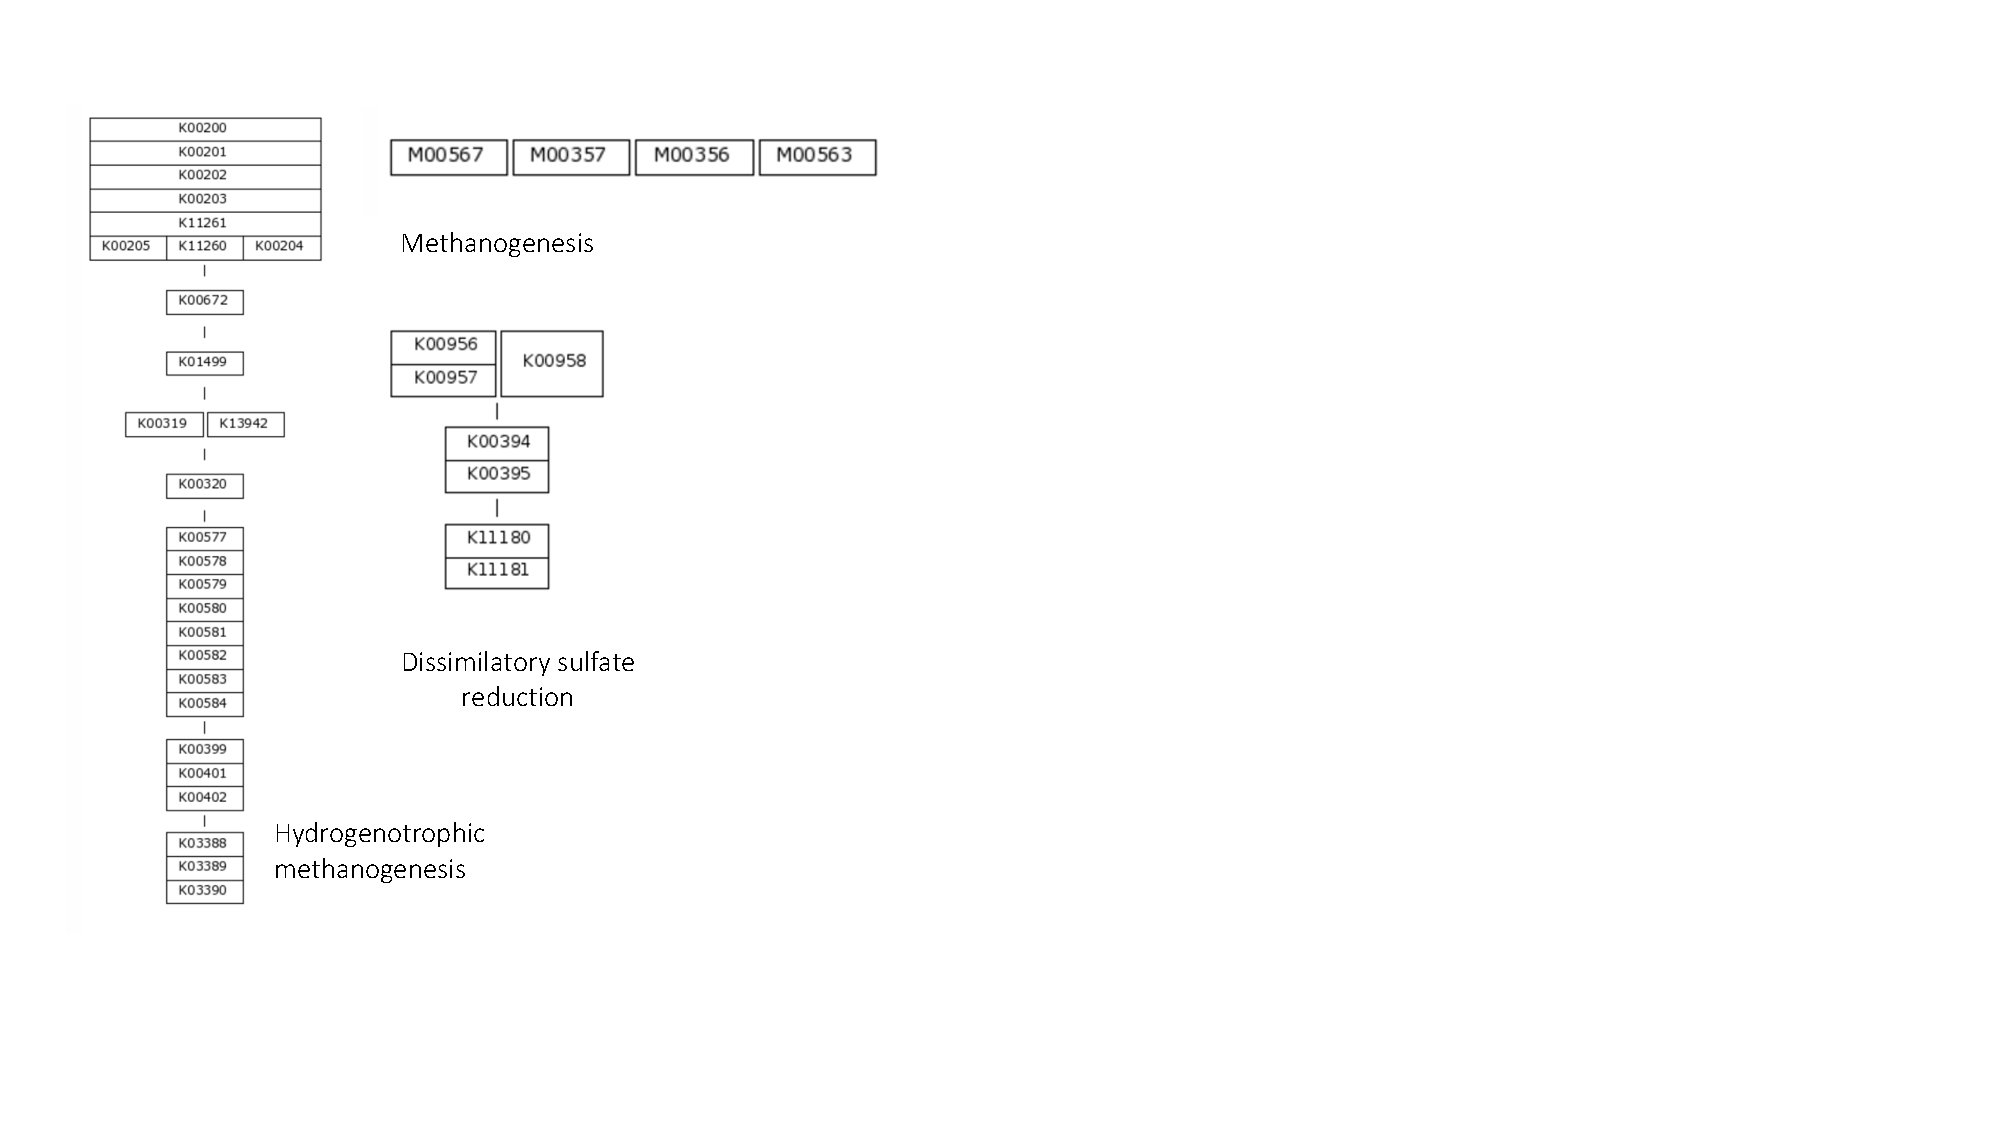
\includegraphics[width=0.6\textwidth]{fig2}
\caption{{\bf KEGG modules for some functions.}
Representations of the KEGG modules corresponding to the FAPROTAX functions shown in Table~\ref{tab1}. Modules are organized into `blocks' of orthologs, typically indicating a protein complex. Orthologs positioned next to each other are `options', i.e. that section of the module is present if any of the adjacent blocks are present.}
\label{fig2}
\end{figure}

\begin{figure}
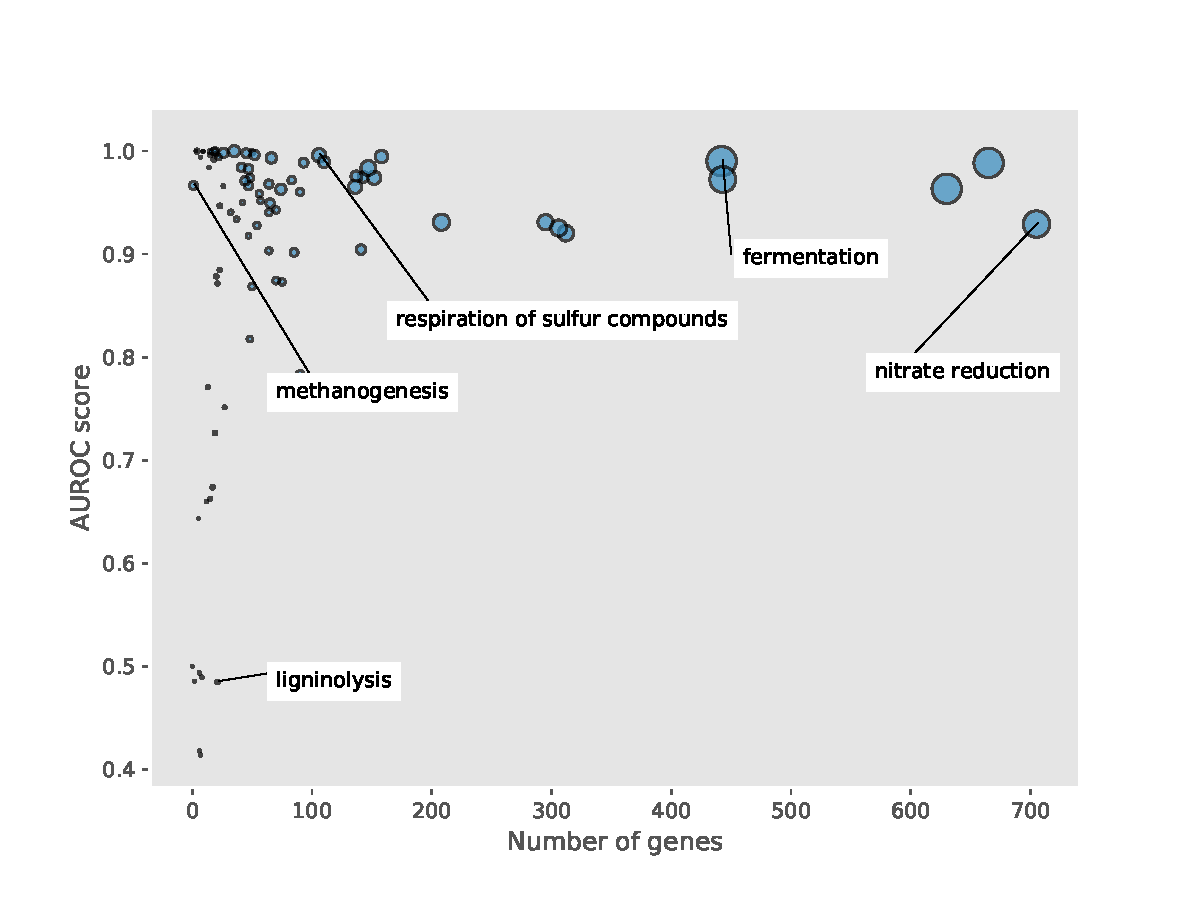
\includegraphics[width=0.7\textwidth]{fig3}
\caption{{\bf Classifier performance and complexity.}
Scatterplot showing the AUROC score of the different classifiers plotted against the number of gene orthologs the classifier uses to make its predictions. Point size is proportional to the number of positive examples in the training set.}
\label{fig3}
\end{figure}

\subsection*{Comparison to KEGG modules}
It is instructive to compare the performance of our classifiers to the use of KEGG modules, where an equivalent module exists for that function, i.e. compare the performance to a `classifier' where an organism is judged capable of a function if it has a complete KEGG module for that function. Table~\ref{tab2} shows the results of this comparison for three FAPROTAX functions with corresponding KEGG modules. Note that the KEGG module method does not require training, so the metrics are over the entire NCBI dataset, whereas for the classifier they are only for the held-out test set. Also, the former method gives only presence/absence of a function rather than a probability, so the AUROC score cannot be calculated, so we use alternative metrics based on classification: the $F_1$ score and the confusion matrix.

It can be seen that our logisitc regression classifier does significantly better than KEGG modules in assigning these functions as they appear in the FAPROTAX database. This suggests that having the enzymes or proteins described in the KEGG module for a function is not in fact a necessary or sufficient condition for actually performing that function, and that other genes are more predictive. However, it is possible that the discrepancy is due instead to inaccuracy in the FAPROTAX database, e.g. species which do perform the functions being missed from the database and therefore getting flagged as false positives with the KEGG method. More work would be needed to fully exclude this possibility.  

\begin{table}
\scriptsize
\begin{tabular}{|c|c|c|c|c|}\cline{2-5}%

 \multicolumn{1}{c|}{} &  \multicolumn{2}{|c|}{\bfseries KEGG modules} & \multicolumn{2}{|c|}{\bfseries Classifier} \\ \hline
 \rowcolor{LightGray} \bfseries module & \bfseries F1 & \bfseries confusion matrix & \bfseries F1 & \bfseries confusion matrix \\\hline
%\rowcolor{VeryLightGray}
sulfate respiration & 0.84 & $\begin{pmatrix}9197 & 53 \\ 6 & 151\end{pmatrix}$ & 0.99 & $\begin{pmatrix}2313 & 0 \\ 1 & 38\end{pmatrix}$\\ \hline
%\rowcolor{VeryLightGray}
nitrate respiration & 0.14 & $\begin{pmatrix}6821 & 2162\\ 224 & 200\end{pmatrix}$ & 0.622 & $\begin{pmatrix}2237 & 9 \\ 54 & 52\end{pmatrix}$\\ \hline
%\rowcolor{VeryLightGray}
hydrogenotrophic methanogensis & 0.756 & $\begin{pmatrix}9281 & 43 \\ 6 & 77\end{pmatrix}$ & 0.923 & $\begin{pmatrix} 2331 & 0\\ 3 & 18\end{pmatrix}$\\ \hline
\end{tabular}

\caption{{\bf Comparison of classifiers to KEGG modules.}
Table showing the performance of using KEGG module presence/absence against LR classifiers for some functions where equivalent KEGG modules exist. Since the KEGG module approach does not give a probability, the AUROC score cannot be used, so the F1 score and confusion matrices are compared.}\label{tab2}
\end{table}

\subsection*{Performance across taxa}
As alluded to above, it is not clear how much the genes being used by the classifiers are actually related to the functions being predicted; they must just be genes that happen to be found in a closely-related set of organisms that happen to all perform the function. The way in which functions are spread over the phylogenetic tree of microorganisms varies between functions~\cite{Martiny2015}, see Figure~\ref{fig4}. As might be expected, closely-related organisms often perform similar functions, with clusters on the tree often sharing the function.

\begin{figure}
\includegraphics[width=0.45\textwidth]{sulfate_resp_tree}
\includegraphics[width=0.45\textwidth]{nitrate_resp_tree}
\caption{{\bf Taxonomic distribution of metabolic traits.}
Taxonomic trees of all prokaryotic NCBI species with full genomes. For training the cross-taxa verison of the classifier, only the Proteobacteria (red section of the tree) were used, and the models were tested on the rest of the tree. Species capable of a) sulfate respiration and b) nitrate respiration are highlighted on the trees.}
\label{fig4}
\end{figure}

To investigate this phenomenon and attempt to find orthologs with real causal associations with functions, we tried training a model on one part of the phylogenetic tree and testing its performance on another. If a classifier can predict phenotype based on genes in a distantly-related, unseen set of organisms, it is likely the genes it is using have a real association with the function. In particular, we tried training our logistic regression models on the Proteobacteria, a large phylum of bacteria, and testing on the rest of the phylogenetic tree of life. Some functions did not have significant numbers of species in each of these sets; we used only functions with at least 5 species in the training set and 5 in the test, leaving 59 functions out of 84. 

As might be expected, our classifiers performed significantly worse in this case, compared to being trained on a random selection of species from throughout the prokaryotic part of the tree of life, see Figure~\ref{fig5}. However, for a significant number of functions the performance of the classsifier is still fairly good, indicating an ability to make predictions which are generalizable to significantly different unseen groups of organisms. 19 functions have an AUROC score greater than 80\%, and 9 greater than 90\%. 

\begin{figure}[!h]
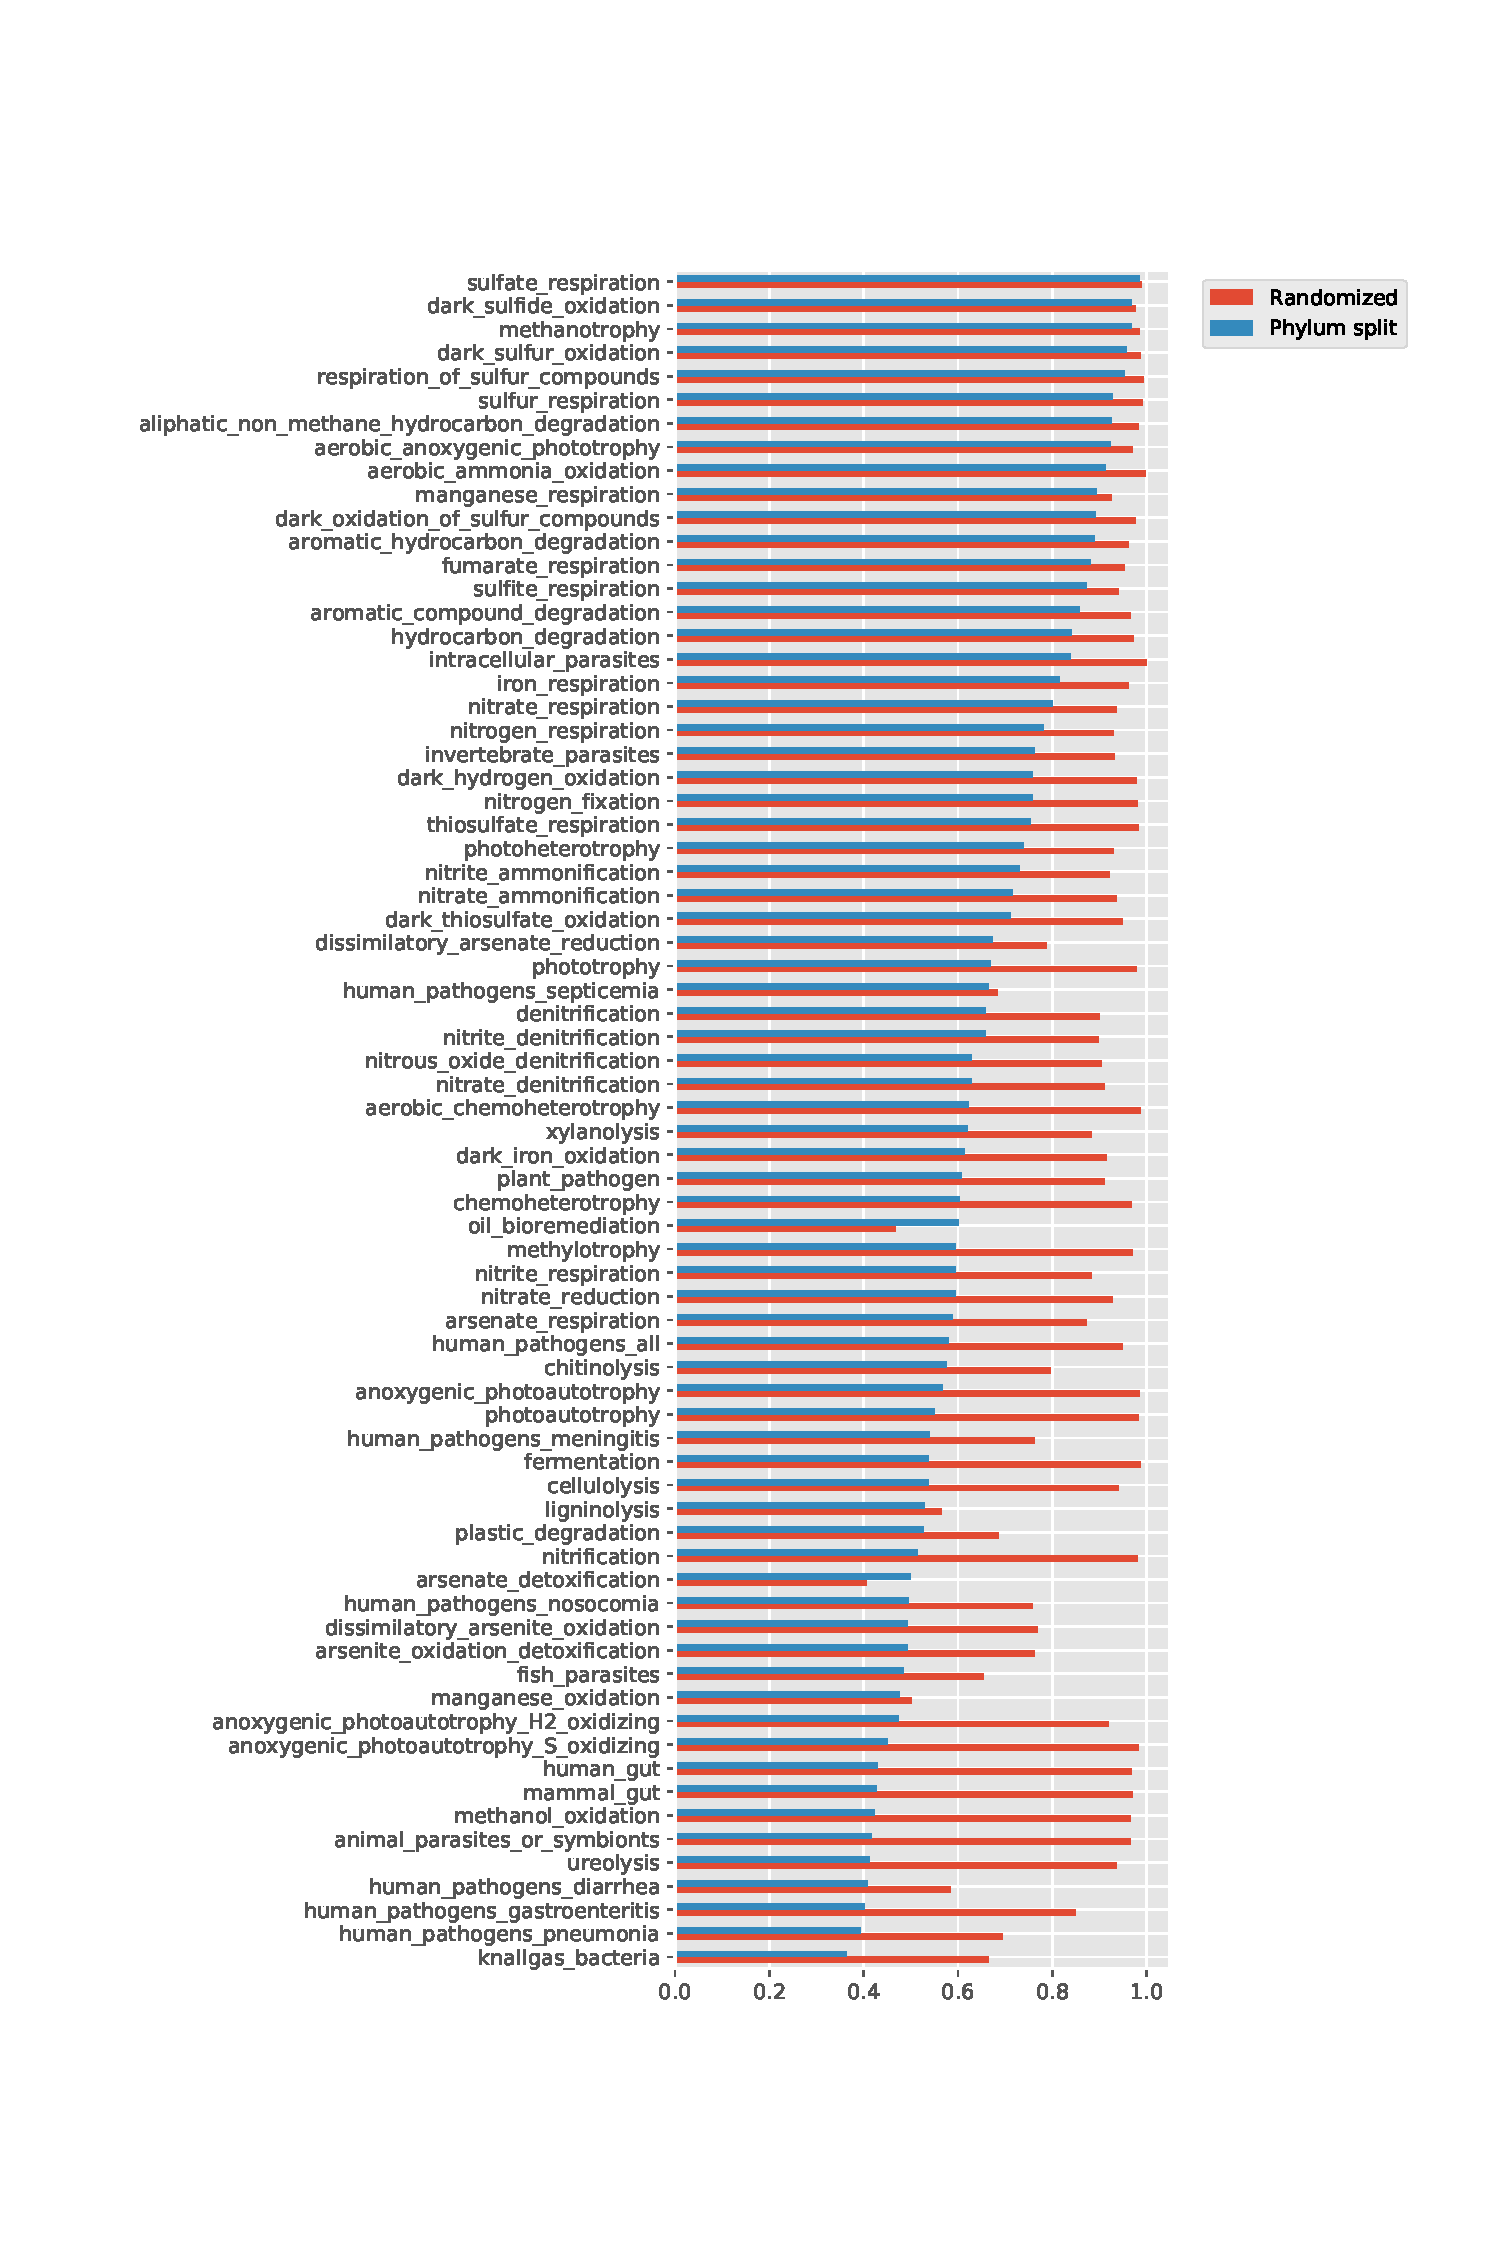
\includegraphics[width=0.9\textwidth]{fig5b}
\caption{{\bf Overall performance of classification algorithm in the cross-taxa case.}
The AUROC score on each classification task (each function) is shown for the LR classifiers based on KOs for the case of random train/test splitting as in Figure~\ref{fig1}, and a classifier trained on the Proteobacteria and tested on all other organisms in the dataset.}
\label{fig5}
\end{figure}

Figure~\ref{fig6} shows a scatter plot of classifier complexity against performance, as in Figure~\ref{fig3}. Notable is that the group of classifiers achieving high accuracy while using a lot of genes is gone: functions such as fermentation and nitrate reduction, which were in this group of classifiers, are now much less accurate. Classifiers which work well in the cross-taxa case all use a relatively small number of genes, less than 150 or so. This suggests that the classifiers using a large number of genes to make predictions in the randomized case may have been using a range of genes found in different closely-related clusters of organisms which all have the target trait, but which may not have a causal relationship with the function.

\begin{figure}
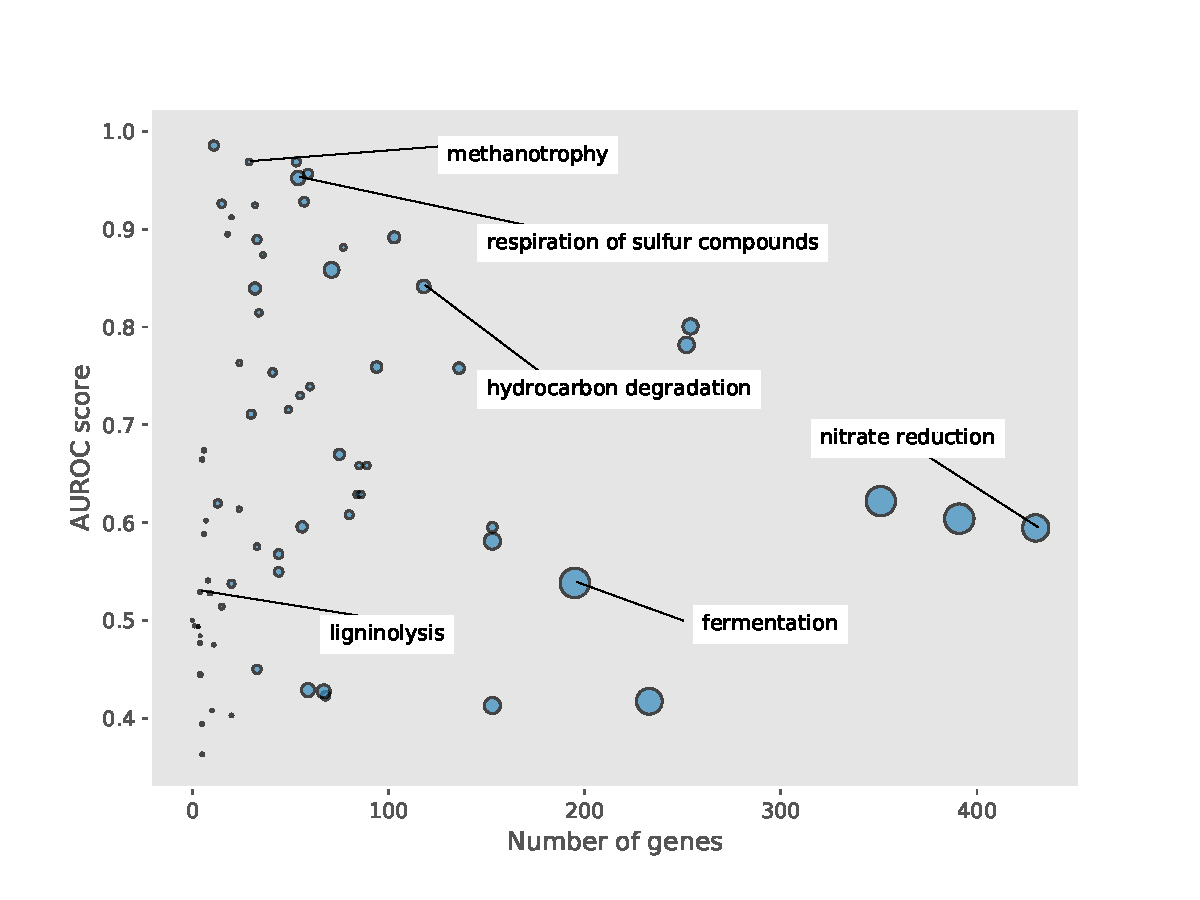
\includegraphics[width=0.7\textwidth]{fig6}
\caption{{\bf Classifier performance and complexity, cross-taxa case.}
Scatterplot showing the AUROC score of the different classifiers plotted against the number of gene orthologs used for the cross-taxa classifiers. Point size is proportional to the number of positive examples in the training set.}
\label{fig6}
\end{figure}

\subsection*{Prediction of MAG phenotypes}
A major aim of trainig these classifiers is to explore the functional capabilities of novel genomes isolated from metagenomic studies. We therefore applied the classifiers trained using the methods above to classify metagenomically assembled genomes (MAGs) from a few different environments. These were laboratory anaerobic digesters, the ocean (from the Tara oceans project~\cite{Zhang2015}), and MAGs from a groundwater aquifer assigned to be members of the so-called `canditate phyla radioation' (CPR)~\cite{Anantharaman2016}. The CPR is a set of bacterial lineages discovered from metagenomic studies consisting of a very large number of proposed novel phyla. These organisms have very small genomes, and may typically live in symbiosis with other organisms (REF).

To do the functional assigments, we used the $\ell$1-regularized loigistic regression classifier described above, with a random train-test splitting and the regularization parameter $C=0.05$, trained using KEGG orthologs on the full NCBI genomes. Figure~\ref{heatmap} shows a heatmap with presence or absence of the different functions for some MAGs assembled from anaerobic digesters and from the global oceans (the Tara project). There are some noticable differences, such more AD MAGS having fermentation and sulfate-metabolism-related functions and fewer having aerobic chemoheterophy. 

\begin{figure}
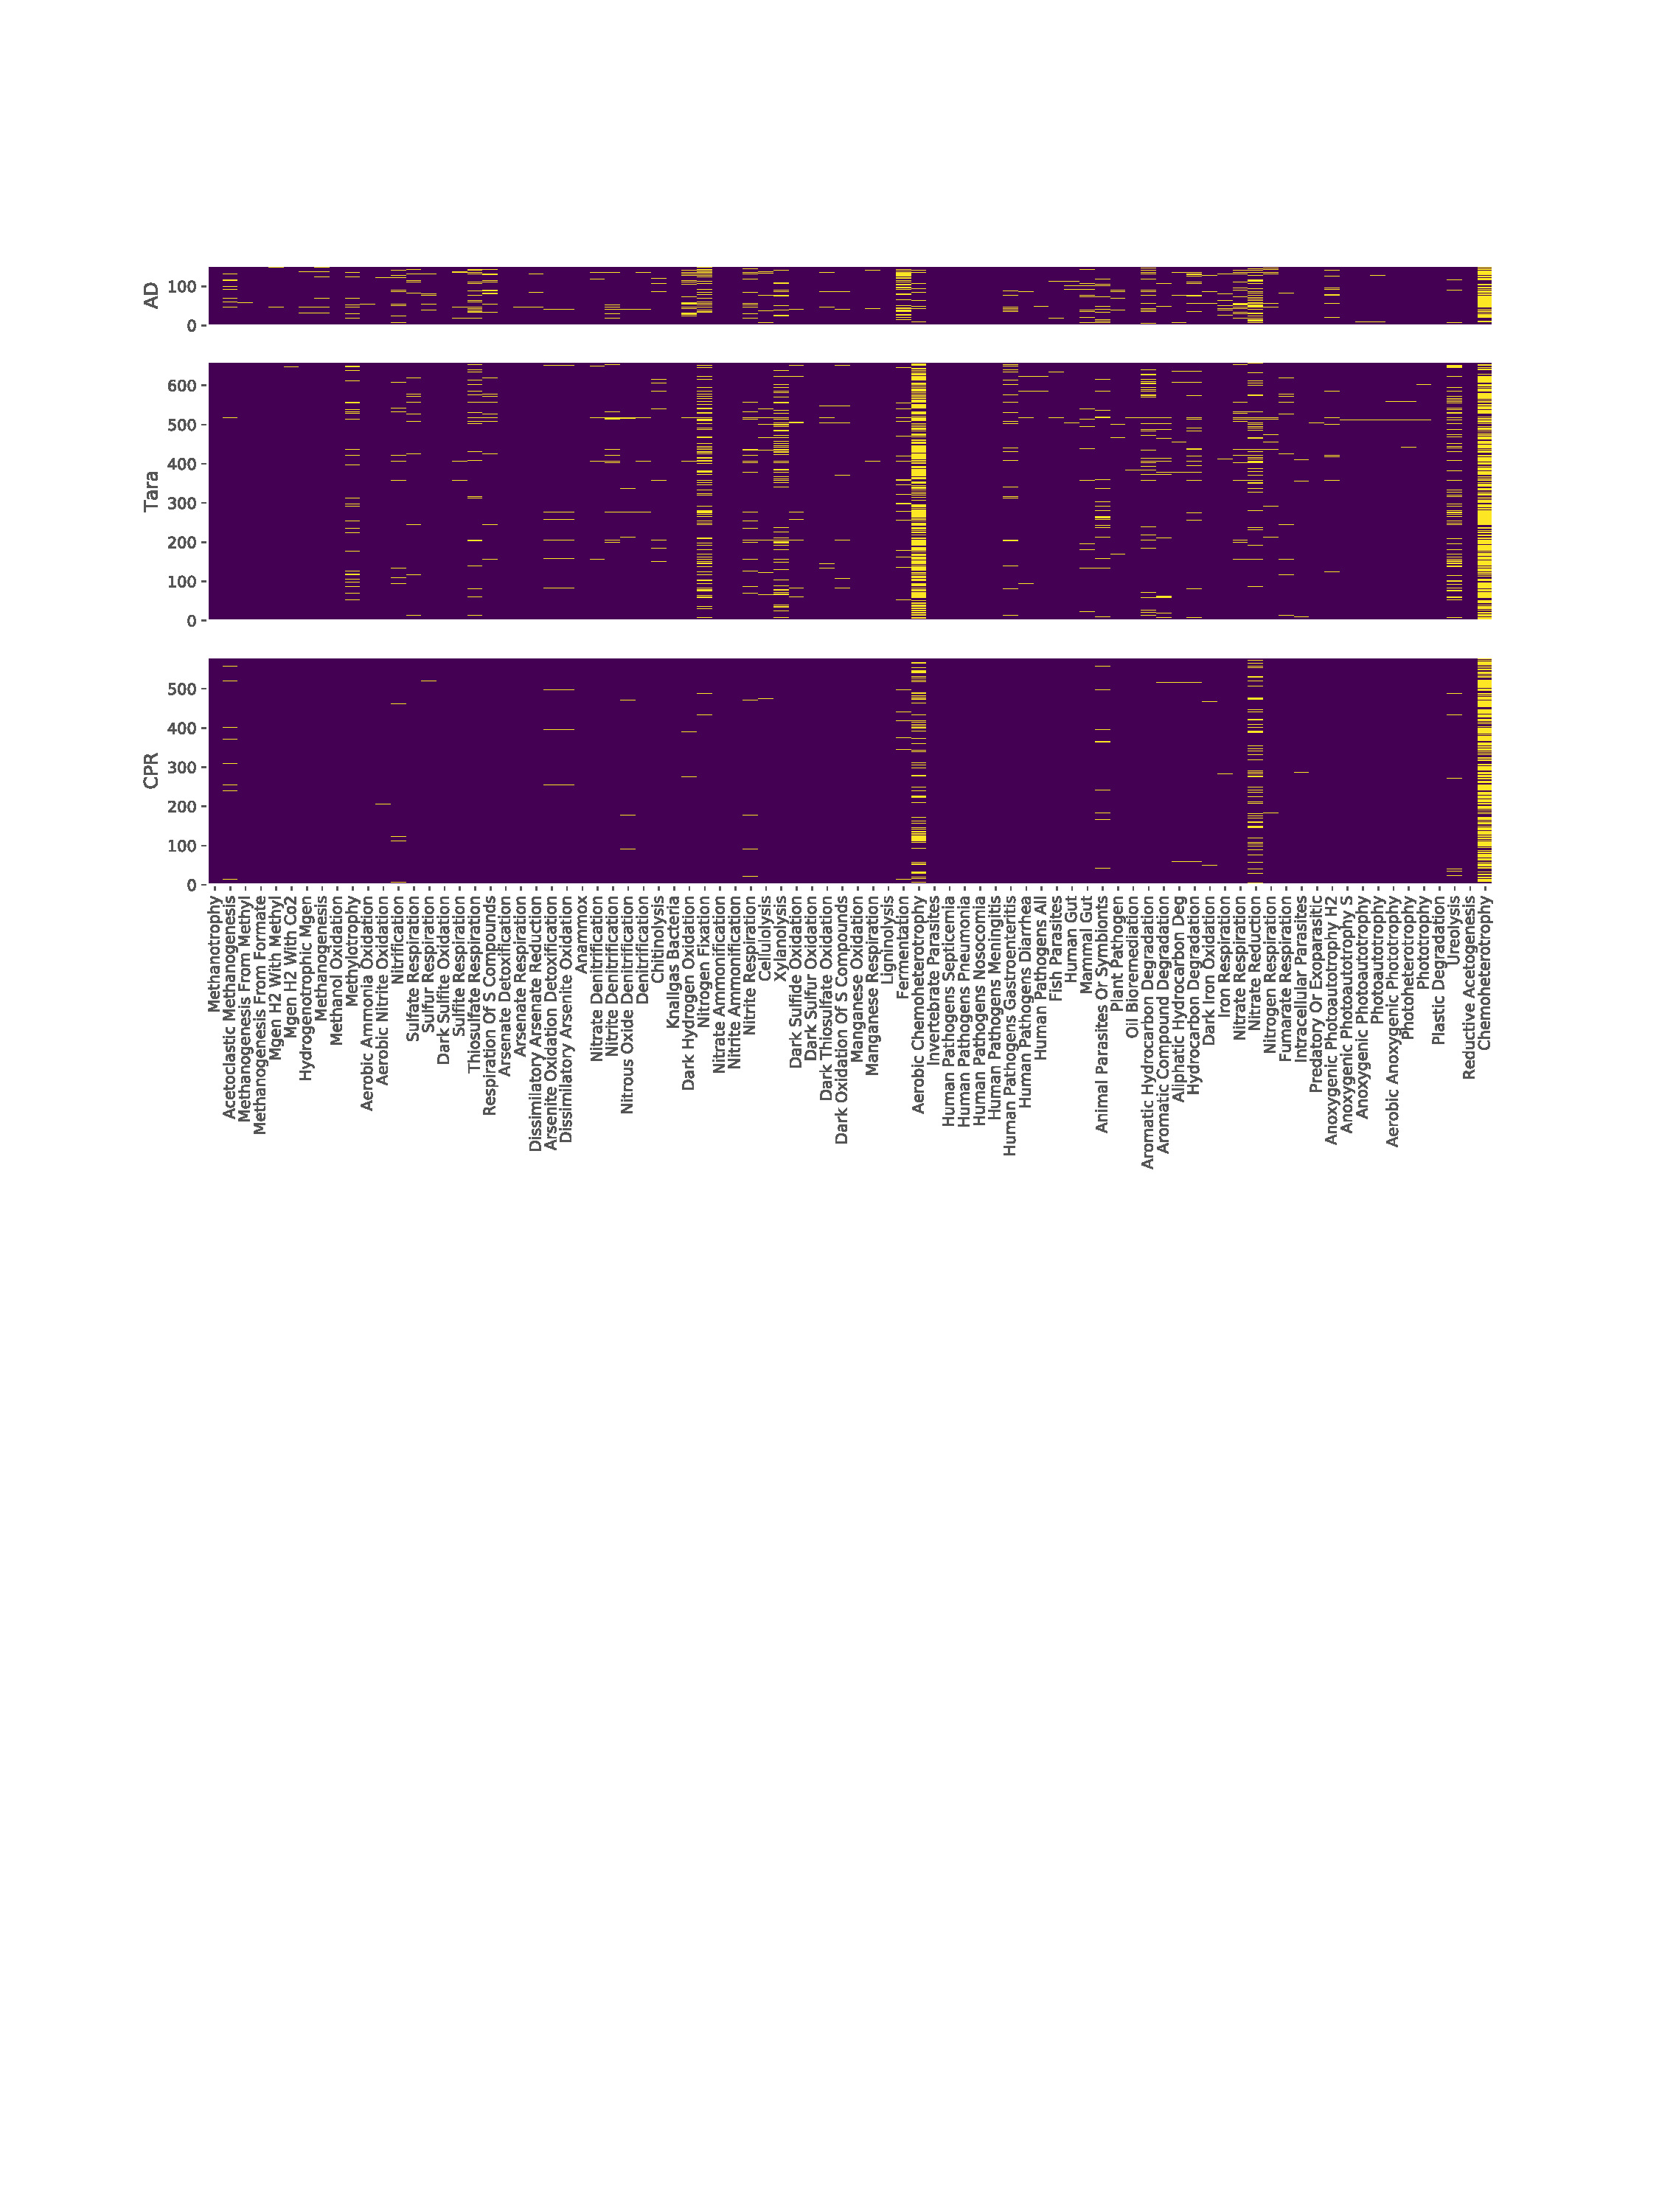
\includegraphics[width=0.9\textwidth]{mag_heatmaps_cpr}
\caption{{\bf Heatmap of presence/absence of fucntions in MAGs.}
Results of running the set of LR classsifiers trained on NCBI genomes on MAGs assembled from three environments: laboratory anaerobic digesters, the ocean and `candidate phyla radiation' (CPR) organisms from an aquifer system.}
\label{heatmap}
\end{figure}

To make these differences clearer, Figure~\ref{mag-compare} is a bar chart showing the proportion of MAGs from the different environments having a function, for some of the most common functions. For many functions, the differences are very significant. 

\begin{figure}
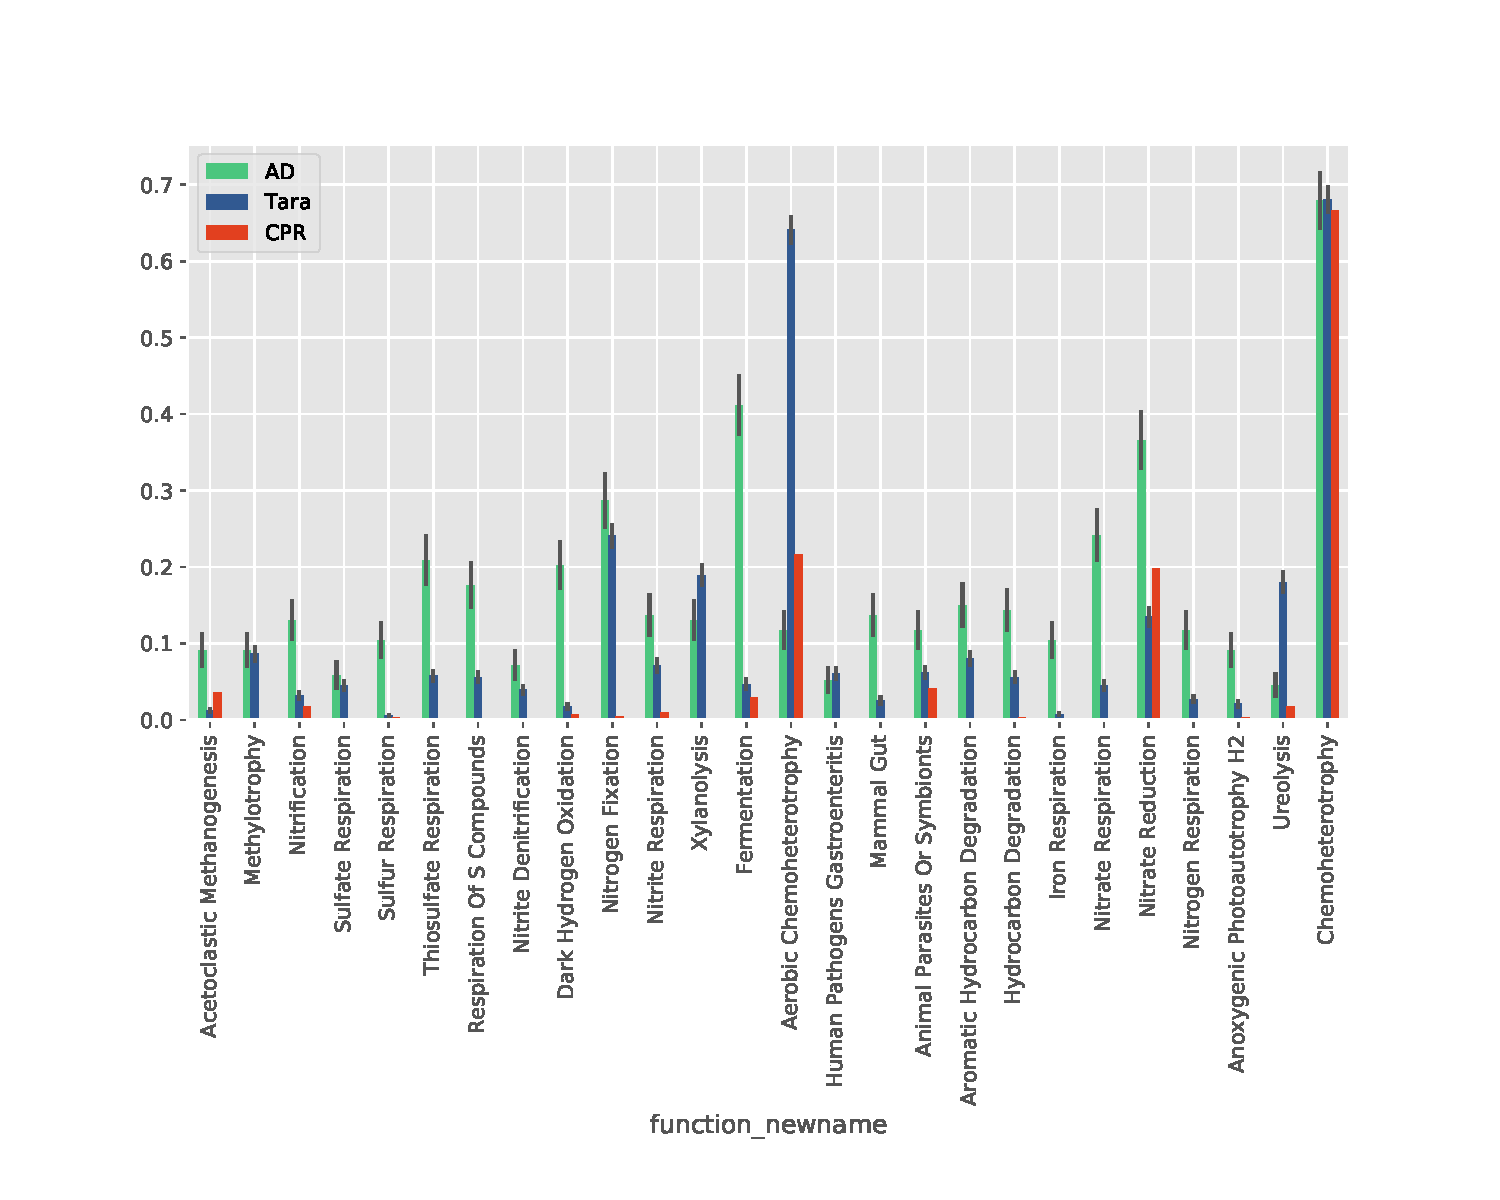
\includegraphics[width=0.9\textwidth]{mag_comparison_bars_cpr}
\caption{{\bf Overall comparison of AD, Tara and CPR MAGs.}
Proportions of MAGS from the environments having a function, for some of the most common functions.}
\label{mag-compare}
\end{figure}

These differences in function might well be expected between these environents. For example, fermentation is very important in the AD process, and aerobic chemoheterotrophy obviously is not as the environment is aerobic. This indicates that the method is acapable of producing useful information about MAGs. The results for the CPR MAGs indicate that these organisms possess significantly fewer functions than those from the other two environments, as would be expected from their very small genome sizes. A few functions do however have significant incidence in this group. Apart from `chemoheterotrophy' and `aerobic chemoheterotrophy', which are very broad categories encompassing a large proportion of all organisms, a few functions associated with nitrogen metabolism, especially nitrate reduction, are noticeably present in the group.

Some of the functional assignments seem strange, for example organisms being classified as acetoclastic or hydrogenotrophic methanogens but not as methanogens, including a significant proportion of CPR organisms (about 3\%), which are bacteria, being classified as acetoclastic methanogens. Looking at the gene orthologs present in these organisms and their taxonomic assignments sheds some light on what is going on here, see Table~\ref{tab3}. For example, some of the acetoclastic methanogens which are misclassified as not being methanogens are missing the \emph{mcrA} ortholog K00399, presumably because the MAGs are incomplete and this gene has been missed. Another example is an organism classified as being a hydrogenotrophic methanogen but not a methanogen. This MAG appears to be from the bacterium \emph{Caldisericum exile}, which is not a methanogen and does not possess \emph{mcrA} (it is an anaerobic, thermophilic bacterium which respires by thiosulfate reduction~\ref{Mori2009}). However, it does possess genes for subunits of the energy-converting hydrogenase A, noted earlier (Table~\ref{tab1}) to be incidative of hydrogenotrophic methanogenesis. Therefore, these discrepancies may be the result either of incomplete MAGs, or of combinations of genes which are rare or unseen in the training set.

\begin{table}
\scriptsize
\csvautotabular{datafiles/methanogen_mag_details.csv}

\caption{{\bf Key genes and predicted functions for MAGs predicted to be methanogens.}
Gene copy numbers for the \emph{mcrA} methanogenesis gene and the energy-converting hyrdogenase A, along with functional predictions, for AD MAGs predicted to be mathanogenic by our algorithm.}\label{tab3}
\end{table}


\section*{Discussion}


\section*{Conclusion}


\section*{Supporting information}

% Include only the SI item label in the paragraph heading. Use the \nameref{label} command to cite SI items in the text.
\paragraph*{S1 Fig.}
\label{S1_Fig}
{\bf Bold the title sentence.} Add descriptive text after the title of the item (optional).



\nolinenumbers

% Either type in your references using
% \begin{thebibliography}{}
% \bibitem{}
% Text
% \end{thebibliography}
%
% or
%
% Compile your BiBTeX database using our plos2015.bst
% style file and paste the contents of your .bbl file
% here. See http://journals.plos.org/plosone/s/latex for 
% step-by-step instructions.
% 

\bibliographystyle{plos2015}
\bibliography{trait_prediction,others}{}

% \begin{thebibliography}{10}

% \bibitem{bib1}
% Conant GC, Wolfe KH.
% \newblock {{T}urning a hobby into a job: how duplicated genes find new
%   functions}.
% \newblock Nat Rev Genet. 2008 Dec;9(12):938--950.

% \bibitem{bib2}
% Ohno S.
% \newblock Evolution by gene duplication.
% \newblock London: George Alien \& Unwin Ltd. Berlin, Heidelberg and New York:
%   Springer-Verlag.; 1970.

% \bibitem{bib3}
% Magwire MM, Bayer F, Webster CL, Cao C, Jiggins FM.
% \newblock {{S}uccessive increases in the resistance of {D}rosophila to viral
%   infection through a transposon insertion followed by a {D}uplication}.
% \newblock PLoS Genet. 2011 Oct;7(10):e1002337.

% \end{thebibliography}



\end{document}

